\section{Purpose Definition}
The iTelos methodology proposes a systematic approach designed to simplify and reduce the effort required to build Knowledge Graphs (KGs), focusing on the specific purpose indicated by the end user. This section provides a detailed overview of the first phase of the methodology.

\subsection{Purpose Formalization}
In this phase, the informal purpose is structured and formalized to guide the development of the Knowledge Graph. Purpose formalization includes the specification of the Domain of Interest, the identification of the main concepts (Concept Identification), the definition of usage scenarios and personas, the formulation of the Competency Questions (CQs) that the Knowledge Graph must be able to answer, and the definition of the conceptual model (ER Model Definition). This step ensures that the design of the KG is aligned with user requirements and provides a clear and consistent framework for the subsequent modeling and implementation phases.
\subsubsection{Informal Purpose}
The purpose of this project is to build a Knowledge Graph (KG) that models the meteorological facilities in the territory and, consequently, the climate and potential climate change in Trentino. The KG will organize information in a structured and accessible way, allowing it to answer precise user queries, such as identifying the locations of weather stations, analyzing temperature and rainfall over recent years, pinpointing areas with the highest temperature increases, and detecting signs of climate change based on historical data.

\subsubsection{Domain of Interest}
The Domain of Interest (DoI) for this project is the Trentino region in 2025, with a particular focus on meteorological phenomena and climate change. The Trentino region exhibits a wide variety of microclimates and weather conditions, ranging from high alpine areas to valleys and lakes, making it an ideal natural laboratory for climate study. The project’s geographic scope covers the entire region, including weather stations, climate sensors, and historical data, enabling a comprehensive analysis of climate patterns.\\
Key features of the domain include:
\begin{itemize}
    \item \textit{Meteorological Monitoring}: Data on temperature, precipitation, humidity, wind, and other variables measured by weather stations distributed throughout the territory.
    \item \textit{Climate Change Monitoring}: Analysis of historical trends and detection of climate variation signals, such as increases in average temperature, changes in precipitation patterns, and local climatic anomalies.
\end{itemize}


\subsubsection{Scenario}
This section presents several usage scenarios, describing the different aspects considered by the project’s purpose.
\begin{itemize}
    \item \textbf{Maria} and her boyfriend, two local researchers, are analyzing precipitation trends in Trentino over the past ten years. They want to identify areas where rainfall has significantly increased or decreased to understand potential impacts on agricultural and forested areas. They use the Knowledge Graph to retrieve historical data from multiple weather stations and compare time series.
    \item \textbf{Giulia}, a climatology student, wants to study the microclimates present in the different valleys of Trentino. She needs access to temperature, humidity, and wind data collected by sensors across the territory to analyze climate variations between alpine and lake areas.
    \item \textbf{Alessandro}, responsible for civil protection, is monitoring climatic anomalies in real time. He aims to quickly identify areas with unusual temperatures or precipitation to plan preventive interventions against landslides or hydrogeological risks.
    \item \textbf{Francesca} and her group of students want to study the impact of climate change on the seasons in Trentino. They need to compare historical data with current measurements to understand the evolution of climatic phenomena, such as delayed snowfall or increased heatwaves.
    \item \textbf{Marco}, a weather enthusiast, uses the Knowledge Graph to explore long-term trends in temperature and precipitation, identify areas with the highest temperature increases, and better understand the signals of climate change in the Trentino region.
\end{itemize}

\subsubsection{Personas}
This section defines a set of real users acting within the previously described scenarios.
\begin{itemize}
    \item \textbf{Maria Bianchi}, 35 years old, a local researcher passionate about meteorology. She is interested in analyzing precipitation trends and the impact of climate change on the territory.
    \item \textbf{Giulia Ferrari}, 23 years old, a climatology student. She enjoys studying microclimates and climate variations between alpine and lake areas.
    \item \textbf{Alessandro Rossi}, 40 years old, responsible for civil protection. He monitors climatic anomalies in real time to prevent landslides and hydrogeological risks.
    \item \textbf{Francesca Romano}, 22 years old, an Erasmus student. She is interested in comparing historical and current data to study the evolution of seasonal climate phenomena.
    \item \textbf{Marco Ricci}, 28 years old, a weather enthusiast. He likes exploring long-term temperature and precipitation trends to better understand the signals of climate change in the Trentino region
\end{itemize}



\subsubsection{Competency Questions (CQs)}
\begin{tabular}{|p{5cm}|p{1cm}|p{10cm}|}
\hline
\textbf{Person} & \textbf{N.o.} & \textbf{Competency Question (CQ)} \\
\hline
Maria Bianchi & 1.1 & Which areas of Trentino have experienced significant increase in annual rainfall over the past decade? \\ Maria Bianchi & 1.2 & Which areas have shown a consistent decrease in precipitation over the past decade? \\ Maria Bianchi & 1.3 & How has the average monthly rainfall evolved in each valley or municipality of Trentino over the last ten years? \\ Maria Bianchi & 1.4 & Are there correlations between changes in rainfall and altitude or proximity to forests and agricultural land?\\ Maria Bianchi & 1.5 & Which weather stations have the most complete historical data on precipitation in Trentino? \\
\hline
Giulia Ferrari & 2.1 & What are the typical temperature ranges and humidity levels in alphine valleys compared to lake areas? \\ Giulia Ferrari & 2.2 & Which areas show microclimatic differences despite geographical proximity? \\ Giulia Ferrari & 2.3 & How does wind speed and direction vary between the Adige Valley and surrounding mountains areas? \\ Giulia Ferrari & 2.4 & Are there correlations between altitude and average annual temperature or humidity? \\ Giulia Ferrari & 2.5 & How stable are microclimates across seasons (winter vs. summer) in different valleys? \\ Giulia Ferrari & 2.6 & Which valleys show the most distinctive microclimatic patterns according to sensor data? \\
\hline
Alessandro Rossi & 3.1 & Which areas of Trentino are currently showing unusually high or low temperatures compared to historical averages? \\ Alessandro Rossi & 3.2 & Are there real-time alerts for abnormal precipitation or snowmelt that could indicate flood risks? \\ Alessandro Rossi & 3.3 & Which zones are currently under potential hydrogeological risk due to recent heavy rainfall? \\ Alessandro Rossi & 3.4 & How do current weather anomalies compare to past extreme events recorded in the KG? \\ Alessandro Rossi & 3.5 & Can the KG highlight areas with recurring climatic anomalies over multiple years? \\ Alessandro Rossi & 3.6 & Which meteorological stations are currently reporting anomalies in temperature or precipitation beyond expected thresholds?\\
\hline
Francesca Romano & 4.1 & How have the average start and end dates of each season changed in Trentino over the past 30 years?\\ Francesca Romano & 4.2 & Has the timing or duration of snowfall periods shifted over time? \\ Francesca Romano & 4.3 & Are heat waves occurring more frequently or lasting longer than in the past? \\ 
\hline
\end{tabular}
\begin{tabular}{|p{5cm}|p{1cm}|p{10cm}|}
\hline
Francesca Romano & 4.4 & How does current spring temperature compare to historical averages from the 1980s and 1990s? \\ Francesca Romano & 4.5 & Which areas show the most significant seasonal shifts (e.g., warmer winters, delayed autumn)? \\ Francesca Romano & 4.6 & How has average precipitation in summer and winter evolved over time?\\
\hline
Marco Ricci & 5.1 & Which areas of Trentino gave recorder the highest temperature increases over the past 50 years? \\ Marco Ricci & 5.2 & How have long-term temperature and precipitation trends evolved across different valleys? \\ Marco Ricci & 5.3 & What are the clearest signals of climate change (e.g., rising temperatures, changing rainfall patterns) in the KG data? \\ Marco Ricci & 5.4 & Are there locations showing evidence of both increased temperature and decreased precipitation? \\ Marco Ricci & 5.5 & Can the KG visualize how average annual temperatures have evolved decade by decade? \\ Marco Ricci & 5.6 & Which weather stations show the most evident long-term warming trends? \\
\hline
\end{tabular}
\subsubsection{Concept Identification}
Concept identification aims to identify which are the main entities and components relevant to the defined purpose. In figure \ref{fig:purpose_formalization_sheet} is reported the Purpose formalization sheet used to collect the main entities in the project.
\begin{figure}[h]
    \centering
    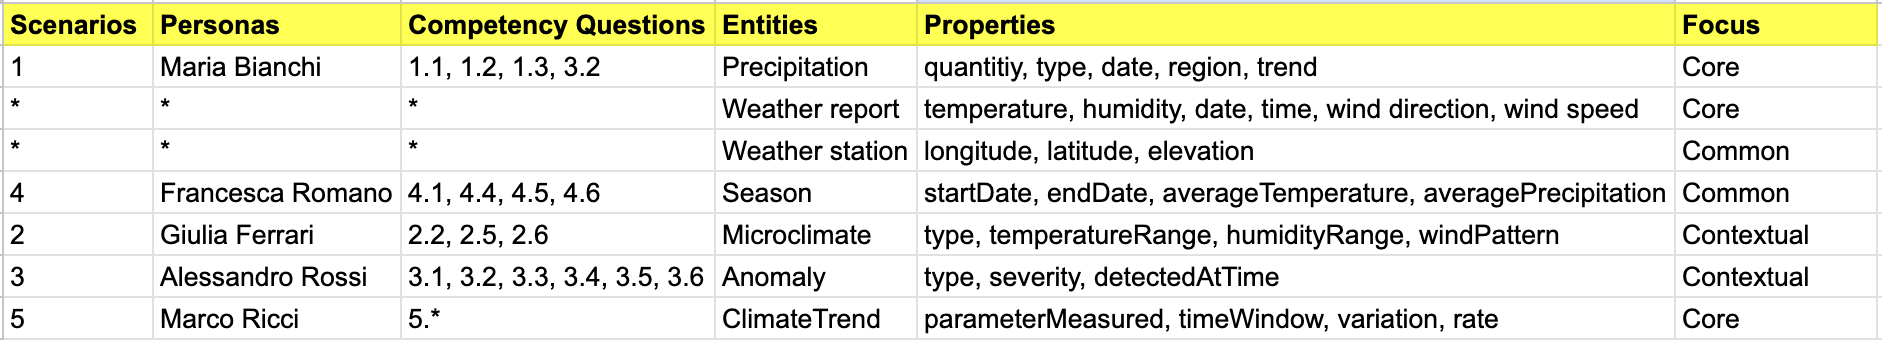
\includegraphics[width=1\textwidth]{../knowdive-files/purpose_formalization_sheet.png}
    \caption{Purpose Formalization Sheet - Concept Identification}
    \label{fig:purpose_formalization_sheet}
\end{figure}
\subsubsection{ER model definition}
\subsubsection{Report}






\subsection{Information Gathering}
This sub-section aims at reporting the execution of the activities involved in Information Gathering. The report, starting from the current section, is organized along two main dimensions. The information gathering sub activities are:
\begin{itemize}
    \item \textbf{KG/KnowDive Data Sources}: these activities aim at collecting the already available KG/KnowDive resources considered for the project. More in detail the resources here described, are "quality and formal" resources (compliant with the quality and reusability guidelines defined by iTleos) which need minimal processing or don't need to be processed or created. The resources described in this section are those that can be already considered to satisfy the project's purpose.
    \begin{itemize}
        \item Knowledge layer:
        \begin{itemize}
            \item Sources description
            \item Formal resources collection;
            \item Formal resources classification over common, core and contextual
        \end{itemize}
        \item Data layer:
        \begin{itemize}
            \item Sources description
            \item Formal resources collection;
            \item Formal resources classification over common, core and contextual
        \end{itemize}
    \end{itemize}

    \item \textbf{External Data Sources}: these activities aim at collecting "informal" resources from sources with a higher level of heterogeneity. The resources collected by the producer process are not necessarily compliant with the iTelos quality and reusability guidelines. Those are the resources that the KG team will transform into quality resources at the end of the process.
    \begin{itemize}
        \item Knowledge layer:
        \begin{itemize}
            \item Sources description
            \item Informal resources collection and scraping;
            \item Informal resources classification over common, core and contextual
        \end{itemize}
        \item Data layer:
        \begin{itemize}
            \item Sources description
            \item Resources collection and scraping;
            \item Resources classification over common, core and contextual
        \end{itemize}
    \end{itemize}
\end{itemize}

\noindent The report of the work done during the above activities of the methodology, has to includes also the description of the  different choices made, with their strong and weak points. In other words the report should provide to the reader, a clear description of the reasoning conducted by all the different team members.


Evaluation - Purpose Definition: A detailed description of the purpose layer evaluation:
\begin{itemize}
    \item Given the data sources gathered - How many scenarios initially considered? How many scenarios finally considered? report each scenario-level details in a table.
    \item Given the data sources gathered - How many users initially considered? How many users finally considered? report each user-level details in a table.
    \item Given the data sources gathered - How many CQs initially considered? How many CQs finally considered? report each CQ-level details in a table.
    \item If valid, report dataset-level formatting and transformations done in this phase?
\end{itemize}